\RequirePackage{fix-cm} % load new fixes to latex
\documentclass{inc/mas}
% \makeindex
%\usepackage[firstpage]{draftwatermark} %uncomment to set document as draft

\usepackage{multirow}
\usepackage{moreverb}
\usepackage{url}
\usepackage{color}

\pdfsubject{}
\keywords{}
\title{Laboration 2 }
\subtitle{Algorithms, TIN092/DIT600\\ Knapsack, Dynamic Programming \\ Group 25}
\affiliation{}
\pdfauthor{Anne-Katrin Krolovitch, Linda Nilsson}
\begin{document}
%\AddToShipoutPicture{{\BackgroundPic}} % uncomment to add a background image
\author{Anne-Katrin Krolovitch \\ 861022-8960\\ \mail{annekatr@student.chalmers.se}\\ \and
Linda Nilsson \\ 840703-4860 \\ \mail{nilind@ituniv.se}\\ \tabularnewline
}
\maketitle
\section{Explanation of the Algorithm} 
 \noindent The problem which needs to be solved is as follows: there are a number of objects, which all have a size and a value, and we have a knapsack which has a capacity. This means that it only can take a certain amount of objects. These objects should amount to a value that is as large as possible.\\

\begin{figure}[h!]
  \centering
      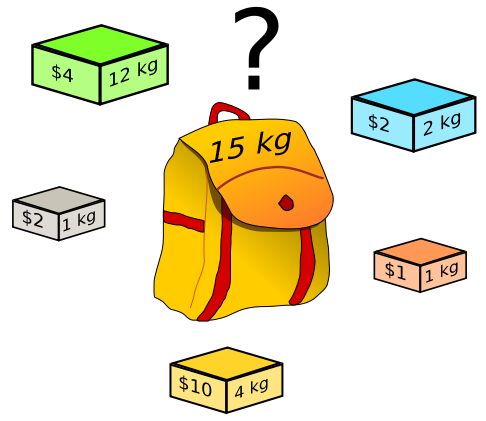
\includegraphics[width=0.5\textwidth]{Knapsack.png}
  \caption{An illustration of the Knapsack problem! \citep{wikipic} }
\end{figure}



\textbf{Definitions:} The number of objects that are in the input file are defined as n, and the capacity of the Knapsack is defined as W.\\

\noindent \textbf{Pseudocode:}
\begin{tabbing}
For \= all the objects in the input file \\
\> fill an \= n by W matrix	\\
\> select the objects that give the highest value and fit into the Knapsack\\
\end{tabbing}

After reading the input file and putting each of these objects into a Tuple which has a weight and a value, the algorithm consists of two parts. First of all, the algorithm fills a matrix (which is going to be a two dimensional array) with the best values the first n tuples can give, which is less than or equal to W. Secondly, it traces which tuples (based on the matrix) gives the highest value and has a weight less than or equal to the capacity of the knapsack. \\ 
 

\section{Algorithm in Pseudocode}

\subsection{Recurrence}
\label{Recurrance}

The recurrence used for finding the best value is defined below. \citep{Tardos} \citep{slides}

$OPT(i,w)$= \Bigg\{ \begin{tabular}{ll} 
0 & if $i$ = 0 \\
$OPT(i-1, w)$ & if $w_i > w$ \\
max \{$OPT(i-1, w), v_i + OPT(i-1, w-w_i )$\} & otherwise\\
\end{tabular}

The first row is the base case, if $i$ is equal to zero the recursion returns. The second case is a check to see if $w_i$ is greater then the capacity, if so it skips object $i$ and continues. The third case on the last row uses the max function on not taking the element versus taking the element. 

\subsection{Pseudocode for finding best value}
In this chapter the algorithm will be explained in more detail. The following is the pseudocode for the function findBestValue(). \citep{Tardos}

\begin{lstlisting}

n = size of the input list
W = capacity of the Knapsack
w1,...,wN = weights of objects in input list
v1,...,vN = values of objects in input list

for w = 0 to W loop
	M[0, w] = 0
end for

for j = 1 to n loop
	M[j, 0] = 0
end for

for i = 1 to n loop
	for w = 1 to W
		if (wi > w)
			M[i, w] = M[i-1, w]
		else
			M[i, w] = max {M[i-1, w], vi + M[i-1, w-wi]}
		end if
	end for
end for

return M[n, W]

\end{lstlisting}

This function is based on the recurrence in the section Recurrence with the difference that it is implemented using loops instead of recurrence and by using the matrix $M$ to remember the results. The first two for loops are part of the pre-processing for the algorithm and initializes the first row and column in the matrix to zeros. The algorithm then checks if the object $i$ in the input list fits in the current capacity, defined as $w$, if it fits it executes a max function of not taking the object and taking the object and stores the max in the matrix as seen in Figure \ref{unmarked_matrix}. 

\begin{figure}[h!]
  \centering
      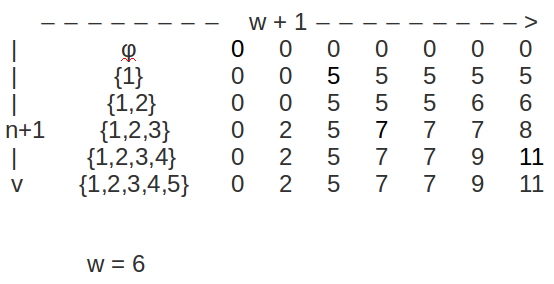
\includegraphics[width=0.5\textwidth]{unmarked_matrix.png}
  \caption{An example of a filled in matrix}
\label{unmarked_matrix}
\end{figure}

\subsection{Pseudocode for tracing best solution}

The second part of the algorithm is to trace the tuples that give the highest value and have a weight less than or equal to the capacity of the knapsack. This pseudocode represents the function printBestSet(). \\ 

\begin{lstlisting}
n = size of the input list containing all the tuples
w = the size of the Knapsack 

for i = n to 1 loop
	if (M[i][weight] is equal to M[i-1][weight])
		do nothing;
	
	else
		w = w - the weight of the object i-1 in the input list
		print the tuples
	end if 
	
end for
\end{lstlisting}

In this part of the algorithm the solution of the problem is reconstructed. This is done by tracing back and comparing the values of the cells in the  matrix. The back tracing starts at the last entry of the matrix (where $i$ = $n$ and $w$ = the size of the Knapsack). Looking at the example matrix Figure \ref{marked_matrix} the algorithm compares the value of place M[i,w] and M[i-1,w] and seeing they both have value 11, object 5 is not included in the optimal solution. If the place of M[i,w] and M[i-1,w] do not have the same value then object $i$ is included in the optimal solution and the algorithm includes this object in the optimal solution and continues to check at place M[i][w-$w_i$] which would be the seven marked in red in the example matrix Figure \ref{marked_matrix}.\\



\begin{figure}[h!]
  \centering
      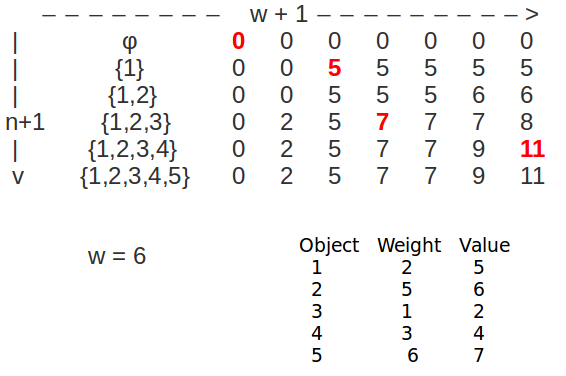
\includegraphics[width=0.5\textwidth]{marked_matrix.png}
  \caption{An example of a matrix for tracing best set solution }
  \label{marked_matrix}
\end{figure}


\section{Correctness Justification}
The justification of the algorithm correctness is done by refering to the induction steps of the recurrence section in chapter 2. \\

\section{Complexity Analysis}
\subsection{Complexity for finding best value}

\begin{lstlisting}

1			n = size of the input list
1			W = capacity of the Knapsack
1			w1,...,wN = weights of objects in input list
1			v1,...,vN = values of objects in input list

W			for w = 0 to W loop
1				M[0, w] = 0
			end for

n			for j = 1 to n loop
1				M[j, 0] = 0
			end for

n			for i = 1 to n loop
W				for w = 1 to W
1					if (wi > w)
1						M[i, w] = M[i-1, w]
					 else
1						if(M[i-1][w] > vi + M[i-1][w-wi])
1							M[i][w] = M[i-1][w];						
						else
1							M[i][w] = vi + M[i-1][w-wi];
						end if
					end if
				end for
			end for

1			return M[n, W]

\end{lstlisting}


\begin{equation}
 5+\sum^W_{w=0}(1)+\sum^n_{j=1}(1)+\sum^n_{i=1}\sum^W_{w=1}(5)
\end{equation}




\subsection{Complexity for tracing best solution}

\begin{lstlisting}
1		n = size of the input list containing all the tuples
1		w = the size of the Knapsack 

n		for i = n to 1 loop
1			if (M[i][weight] is equal to M[i-1][weight])
				do nothing;
	
			else
1				w = w - the weight of the object i-1 in the input list
1				print the tuples
			end if 
	
		end for
\end{lstlisting}

\begin{equation}
 2+\sum^n_{i=1}(3)
\end{equation}

\subsection{Total Complexity}
\begin{equation}
\begin{split}
 5+\sum^W_{w=0}(1)+\sum^n_{j=1}(1)+\sum^n_{i=1}\sum^W_{w=1}(5)+ 2+\sum^n_{i=1}(3)= \\
7+W-0+1+n-1+1+(n-1*(W-1+5))+n-1+3= \\
7+W+1+n+(n-1*(W+4))+n+2= \\
W+2n+10(n-1*(W+4))= \\
n*W+W+2n+cn \in O(n*W)
\end{split}
\end{equation}


\section{Performance Test}

The time for each test is measured in milliseconds. The tests were done by using java.lang.System.currentTimeMillis() to get one start time as the first thing done in the findBestValue method in the algorithm, and one stop time in the printBestSet method after the best set is recoverd but before the result is printed to the screen. The resulting execution time was calculated by subtrackting the the start time from the stop time to get a result of how long the algorithm was executing with the different input files. The result of the previous lab with exhaustive search is also included, n/a in this table means that the algorithm could not deal with that many input objects and ran out of memory. \\

\begin{table}
\begin{center}
\caption{Test result exhaustive search}
\begin{tabular}{|l|l|l|} \hline
Objects &Capacity &Execution time\\ \hline
\multirow{3}{*}{10} & 6 & 11 \\
& 20 & 11 \\
& 35 & 10 \\ \hline
\multirow{3}{*}{15} & 6 & 57 \\
& 20 & 61 \\
& 35 & 59 \\ \hline
\multirow{3}{*}{20} & 6 & 1460 \\
& 20 & 1447 \\
& 35 & 1445 \\ \hline
\multirow{3}{*}{50} & 30 & n/a \\
& 80 & n/a \\
& 120 & n/a \\ \hline
\multirow{3}{*}{100} & 30 &  n/a\\
& 80 & n/a \\
& 120 & n/a \\ \hline
\multirow{3}{*}{500} & 120 & n/a \\
& 250 & n/a \\
& 400 & n/a \\ \hline
\multirow{3}{*}{2000} & 400 & n/a \\
& 800 & n/a \\
& 1500 & n/a \\ \hline
\multirow{3}{*}{8000} & 1500 & n/a \\
& 4000 & n/a \\
& 7000 & n/a \\ \hline
\end{tabular}
\end{center}
\end{table}

\begin{table}
\begin{center}
\caption{Test result dynamic programming}
\begin{tabular}{|l|l|l|} \hline
Objects &Capacity &Execution time\\ \hline
\multirow{3}{*}{10} & 6 & 0 \\
& 20 & 0 \\
& 35 & 1 \\ \hline
\multirow{3}{*}{15} & 6 & 0 \\
& 20 & 0 \\
& 35 & 1 \\ \hline
\multirow{3}{*}{20} & 6 & 0 \\
& 20 & 0 \\
& 35 & 1 \\ \hline
\multirow{3}{*}{50} & 30 & 7 \\
& 80 & 8 \\
& 120 & 8 \\ \hline
\multirow{3}{*}{100} & 30 & 7 \\
& 80 & 9 \\
& 120 & 11 \\ \hline
\multirow{3}{*}{500} & 120 & 30 \\
& 250 & 43 \\
& 400 & 40 \\ \hline
\multirow{3}{*}{2000} & 400 & 94 \\
& 800 & 104 \\
& 1500 & 108 \\ \hline
\multirow{3}{*}{8000} & 1500 & 212 \\
& 4000 & 279 \\
& 7000 & 1046 \\ \hline
\end{tabular}
\end{center}
\end{table}
\newpage
\appendix
\section{Compile and run program}
\noindent Compile the program with 'javac Knapsack.java'\\ 
\noindent Run the compiled program with 'java Knapsack ``inputfile.txt''' where inputfile is the name of the input file. If no input file is provided, the instance 3 input file given in the problem is used as default. 

% References define a context
\bibliographystyle{apalike} %apalike, abbrv, acm, alpha, apalike, ieeetr, plain,
%siam,unsrt
\bibliography{ref}
%\printindex
\end{document}
